%%%%%%%%%%%%%%%%%%%%%%%%%%%%%%%%%%%%%%%%%%%%%%%%%%%%%%%%

%%%%%%%%%%%%%%%%%%%%%%%%%%%%%%%%%%%%%%%%%%%%%%%%%%%%%%%%
\section{Materials and Methods}
%%%%%%%%%%%%%%%%%%%%%%%%%%%%%%%%%%%%%%%%%%%%%%%%%%%%%%%%
%%%%%%%%%%%%%%%%%%%%%%%%%%%%%%%%%%%%%%%%%%%%%%%%%%%%%%%%
%
OWP FIM is a fully operational pipeline of software tools to help acquire datasets, cache hydrofabrics, produce FIMs, and evaluate results.
%
%%%%%%%%%%%%%%%%%%%%%%%%%%%%%%%%%%%%%%%%%%%%%%%%%%%%%%%%
\subsection{Software Dependencies and Architecture}
\label{ssec:software}
%%%%%%%%%%%%%%%%%%%%%%%%%%%%%%%%%%%%%%%%%%%%%%%%%%%%%%%%
%
OWP FIM exclusively utilizes free and open source software dependencies including Python 3, GDAL, TauDEM, Geographic Resource Analysis Support System (GRASS), GNU Parallel, and MPICH \cite{python382,gdal2020,tarboton2005terrain,grass2020,tange2015gnu,amer2021mpich}.
Within the Python 3 ecosystem, many common packages are employed including but not limited to RichDEM, GeoPandas, Rasterio, Rasterstats, and Numba \cite{barnes2018richdem,jordahl2014geopandas,lam2015numba}. 
To simplify setup and enhance portability across host operating systems OWP FIM packages all dependencies up in a Docker image (\url{https://docs.docker.com/engine/install/}). 
A user only needs to install Docker on their host machine and build the image from the provided recipe. 
Source code is made available for this project on GitHub \cite{inundationMapping2022}. 

The pipeline is discretized into key areas that a user can interact with to reproduce the results of this study. 
Preprocessing acquires and prepares datasets for production of the FIM hydrofabric. 
The FIM hydrofabric is defined as the datasets required to make an inundation map from discharges including the relative elevation model (REM) or HAND grid, the catchments in vector and raster form, and the hydro-table (contains synthetic rating curves and cross-walk information).
Functionality is included to turn FIM hydrofabric and streamflows into inundation maps represented in both binary and depths.
Lastly, a test suite includes means of calculating evaluation metrics compared to a variety of preprocessed test case data.
A user should visit the Readme.md page on GitHub for more information on how to acquire the datasets and reproduce the pipeline.
%
%%%%%%%%%%%%%%%%%%%%%%%%%%%%%%%%%%%%%%%%%%%%%%%%%%%%%%%%
\subsection{Datasets}
\label{ssec:datasets}
%%%%%%%%%%%%%%%%%%%%%%%%%%%%%%%%%%%%%%%%%%%%%%%%%%%%%%%%
%
Data sources used within OWP FIM are publicly available from a variety of government sources including the USGS, NWC, Federal Emergency Management Agency (FEMA), and US Army Core of Engineers (USACE) to enhance reproducibility and collaboration among government, academia, and industry.
Instructions for accessing data are provided on the project's GitHub page via an Amazon Web Services (AWS) S3 bucket furnished by Earth Science Information Partners (ESIP) \cite{esipData2022}.
The National Hydrography Dataset Plus High Resolution (NHDPlusHR) Beta Version is the latest hydrography dataset used for land surface hydrologic modeling in the US \cite{moore2019user}.
We utilized a series of data products from the NHDPlusHR including the BurnLineEvents \cite{nhdplus2022vectors}, Value Added Attributes (VAA) \cite{nhdplus2022vectors}, Water Boundaries (WBD) or HUC Layers \cite{nhdplus2022wbd}, and the DEM elevation rasters \cite{nhdplus2022dems}.
It is used in conjunction with the hydrofabric of the NWM V2.1 to help define flowlines for OWP FIM while the NWM hydrofabric is also used to define reservoirs for exclusion and catchments to cross-walk to for forecasting purposes \cite{nwm2022hydrofabric}.
For enforcing levee data into the DEMs, the USACE NLD is used to burn feature elevations \cite{engineers2016national}.
Since NHDPlusHR datasets extend beyond land borders into sea and Great Lake regions, we used the land-sea border from OpenStreetMap (OSM) and the land-lake border from Great Lakes Hydrography Dataset (GLHD) to exclude those areas from production of FIMs \cite{osm2021landsea,GreatLakesHydrographyDataset}.
Additionally, the Base Level Engineering (BLE) datasets within FEMA Region 6 spanning parts of 9 states including Colorado, New Mexico, Texas, Oklahoma, Kansas, Arkansas, Louisiana, Missouri and Mississippi at two recurrence intervals, 1\% (100 year) and 0.2\% (500 year), are used as validation in this study and furnished by the Interagency Flood Risk Management (InFRM) consortium \cite{fema2021base,fema2021estimated}. 
These BLE datasets are provided at the watershed scale (HUC8) utilizing best available simulations and DEMs.
The full input datasets presented by source are listed in Table \ref{tab:data}.
%
\begin{sidewaystable}
\caption{Data sources, names, descriptions, and citations.}
\label{tab:data}
\centering
\begin{tabular}{|p{1.75cm}|p{4cm}|p{11cm}|p{5cm}|}
%\begin{tabular}{l c c}
\hline
Source & Name & Description & Citations\\
\hline
USGS & NHDPlusHR BurnLineEvents & Stream lines used by NHDPlus HR for hydro-enforcement & \cite{nhdplus2022vectors} \\
\hline
USGS & NHDPlusHR Value-Added Attributes & Database of additional attributes associated with the BurnLineEvents that enhance navigation, analysis, and display & \cite{nhdplus2022vectors} \\
\hline
USGS & NHDPlusHR DEM & DEM used for NHDPlus HR at 1/3 arc-second (10 m) spatial resolution and vertical units in centimeters & \cite{nhdplus2022dems} \\
\hline
USGS & NHDPlusHR WBD & Water Boundaries (WBD) or HUCs used for spatial processing units & \cite{nhdplus2022wbd} \\
\hline
NOAA-OWP & NWM Streams & Stream network center lines used by NWM for routing and forecasting. & \cite{nwm2022hydrofabric} \\
\hline
NOAA-OWP & NWM Catchments & Surface drainage area corresponding to each reach in the NWM. & \cite{nwm2022hydrofabric} \\
\hline
NOAA-OWP & NWM Waterbodies & Waterbodies considered by the NWM as reservoirs or lakes. & \cite{nwm2022hydrofabric} \\
\hline
USACE & NLD & Levee database of locations and elevations & \cite{engineers2016national} \\
\hline
OSM & Land-Sea Border & Border of land and sea. & \cite{osm2021landsea} \\
\hline
GLHD & Land-Great Lakes Border & Border of land and Great Lakes. & \cite{GreatLakesHydrographyDataset} \\
\hline
InFRM & Cross-Sections & HEC-RAS 1-D cross-sections used for modeling in BLE datasets. Includes discharges for 1\% and 0.2\% recurrence interval events. & \cite{fema2021estimated} \\
\hline
InFRM & Flood Inundation Extents & Inundation depths produced by InFRM BLE HEC-RAS 1D for 1\% and 0.2\% recurrence interval events. & \cite{fema2021estimated} \\
\hline
\end{tabular}
%\end{table}
\end{sidewaystable}
%
Areas with all the required data (from the NWM and the USGS) are labeled as the FIM domain which includes 2,188 HUC8s for the FR and GMS networks and 1,604 HUC8s for the MS method. 
These methods will be explained more later.
An enhancement of OWP FIM over previous HAND based FIM versions is the support for Hawaii and Puerto Rico which the NWM V2.1 will cover.
%
%%%%%%%%%%%%%%%%%%%%%%%%%%%%%%%%%%%%%%%%%%%%%%%%%%%%%%%%
\subsection{Hydro-conditioning}
\label{ssec:hydro_conditioning}
%%%%%%%%%%%%%%%%%%%%%%%%%%%%%%%%%%%%%%%%%%%%%%%%%%%%%%%%
%
The DEM is subject to a series of hydro-conditioning procedures to enhance its suitability for riverine flood inundation mapping with HAND. 
These techniques are specific for making OWP FIM and differ from the conditioning methods used by the NHDPlusHR Beta \cite{moore2019user}.
HAND inherently requires all areas eligible for inundation to drain to the designated drainage network so DEMs must undergo significant manipulation to make this the case.
In other words, all areas within a given processing unit for HAND must have monotonically decreasing elevations if we wish to have them be eligble for flooding.
Hydro-conditioning is implemented to obtain many objectives including enforcing the location of hydrologically relevant features such as flowlines, lakes, or drainage divides whether natural or anthropogenic. 
It can also be used to simulate more accurate bathymetry which is not accounted for in the 10 m DEM \cite{gesch2002national}.

Specifically within the context of OWP FIM, the hydro-conditioning operations that take place in sequential order are presented. 
Prior to any hydro-conditioning, all input datasets must be subset from their original spatial domain scales into the processing units of size HUC8. 
The subsetting is done by spatial query for the cases of the levees, DEM, and NWM hydrofabric while the NHDPlusHR BurnLineEvents are subset via attribute query for the given reach code's membership in the processing unit.
Hydro-conditioning raster operations take place on buffered boundary definitions to avoid edge contamination and effects \cite{lindsay2013measuring}. 
%
%%%%%%%%%%%%%%%%%%%%%%%%%%%%%%%%%%%%%%%%%%%%%%%%%%%%%%%%
\subsubsection{Stream Network Enforcement} 
\label{ssec:stream_network_enforcment}
%
The location of the stream network is enforced to ensure general agreement with established stream networks especially the placement of the NWM network which is used for forecasting the stream flow inputs.
The NHDPlusHR Beta Burnline Event layer is used to enforce stream locations in the NHDPlusHR workflow so it is also used here for hydro-enforcement \cite{moore2019user}. 
However, to better match the drainage density of the NWM V2.1 stream network which is based on the NHDPlus MR, the Burnline Events are pruned utilizing a nearest neighbor search around the NWM flowlines.
For every NWM headwater segment a headwater point is derived and linearly interpolated to the nearest Burnline Event segment.
Burnline Event headwater segments are split at the adjusted headwater point to match NWM flowlines.
The resulting pruned NHDPlusHR stream network is what gets hydro-enforced in subsequent operations.
This procedure is best illustrated in Figure \ref{fig:stream_density_pruning} which shows that the pruned NHDPlusHR network corresponds to the full density NHDPlusHR network at NWM V2.1 headwater locations only. 
Additionally, the NHDPlusHR pruned headwaters are later used for seeding a new FIM drainage network that best agrees with the DEM after all hydro-conditioning takes place.
This results in a stream network that has the same density as the NWM V2.1 flowline network but utilizes the locations of the NHDPlusHR Beta BurnLineEvents. 
%
\begin{figure}[h!]
\centering
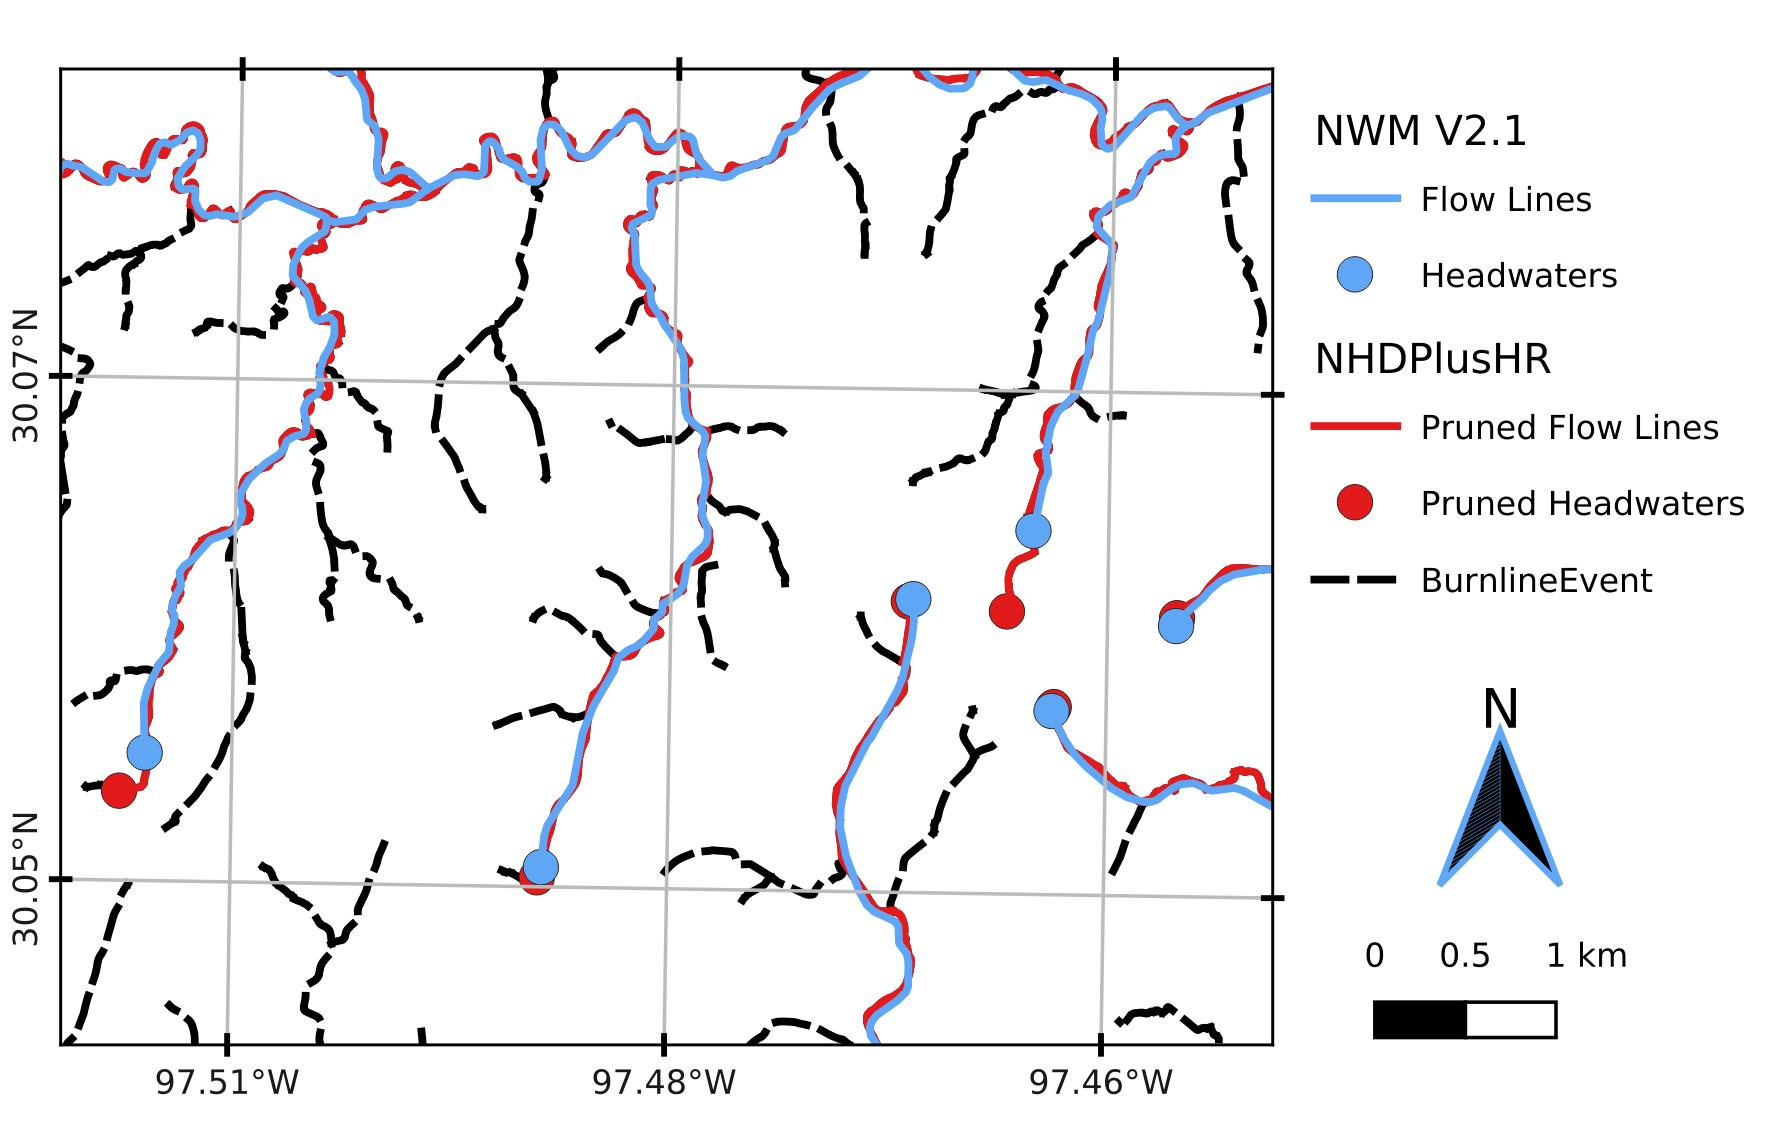
\includegraphics[scale=1.0]{figures/headwaters.jpg}
\caption{Pruning of NHDPlus HR Beta Burnline Events (dotted black) to NWM V2.1 stream density (blue) using nearest neighbor selection and linear interpolation. Resulting stream network (red) matches the drainage density of NWM V2.1 while corresponding spatially with the NHDPlusHR Burnline Events.}
\label{fig:stream_density_pruning}
\end{figure}
%

The pruned stream network is then utilized to hydro-enforce the DEM with a methodology developed by \citeA{hellweger1997agree} known as the AGREE DEM Surface Reconditioning System. 
The AGREE algorithm seeks to burn artificially deep thalweg elevations by a uniform value known as sharp drop. 
The modification continues by excavating an area of a given buffer distance from the thalweg by a depth proportional to the distance from the channel given by the smooth drop. 
The resulting enforcement of the thalweg and general bathymetric region results in a cross-section resembling a trapezoidal shape with a significantly lower elevation along the thalweg line only.
In total, the AGREE algorithm requires three parameters including the buffer distance, smooth drop, and sharp drop which were set to fixed values of 70m, 1000m, and 10m, respectively.
While the value of these parameters are critical to the inundation extents produced, especially for lower flow rates, finding their optimal value for OWP FIM was not done since it was out of the main scientific scope of this article.
Using the AGREE method as opposed to simple thalweg burning techniques helps prevent distortions in the delineation of streams as well as the catchment boundaries \cite{saunders1995grid,saunders1996gis,mizgalewicz1996modeling,hellweger1997agree,quenzer1998gis,baker2006comparison}.
\citeA{baker2006comparison} noted AGREE produced satisfactory results when compared to other enforcement especially when computational costs are considered. 
Downsides to the technique include the possibility of exhibiting parallel streams where the burned stream and real stream are both represented \cite{hellweger1997agree,saunders1999preparation} and some distortion of the catchment boundaries can also be observed \cite{saunders1999preparation,saunders1996gis}. Some of these drawbacks are later addressed by additional conditioning techniques later on.
%
%%%%%%%%%%%%%%%%%%%%%%%%%%%%%%%%%%%%%%%%%%%%%%%%%%%%%%%%
\subsubsection{Levee Enforcement}
%
Coarse DEM's at 10m, 30m, and higher resolutions can lack sufficient representation of fine grain features such as embankments, floodwalls, and closure structures \cite{arundel2018assimilation,dobbs2010evaluation,wang2005comparison,sanders2007evaluation}.
In order to better represent the influences of these features upon hydraulics and inundation extents, the National Levee Database (NLD) published by USACE was used to enforce elevations within the 10 m DEM.
The elevations found in the NLD are burned into the DEM if those elevations were found to exceed those already in place.
%
%%%%%%%%%%%%%%%%%%%%%%%%%%%%%%%%%%%%%%%%%%%%%%%%%%%%%%%%
\subsubsection{Depression Filling}
\label{sssec:depression_filling}
%
Local depressions are naturally occurring features of a DEM but must be addressed if a connected drainage network with continuous catchments are to be derived for flood modeling purposes.
The conditioned DEM was removed of depressions by filling areas with pits while preserving the stream and levee information previously enforced.
Priority-Flood developed by \citeA{barnes2014priority} is an algorithm for filling said depressions and shown to have improved performance over early works in the field by \citeA{jenson1988extracting} implemented in \citeA{tarboton2005terrain} as well as \citeA{planchon2002fast}.
The depression filling algorithm used in our pipeline is a Priority-Flood variant developed by \cite{zhou2016efficient} with enhanced single-thread performance and a time complexity of O(n log n) for floating point grids.
This performance was enabled by limiting the processing queue with a region-growing method to exclude many of the slope cells \cite{zhou2016efficient}.
The depression technique employed here does leave the existence of flat regions where pits existed a prior thus later requiring the need for resolving these flats.
The enhanced variant of Priority-Flood is implemented and made available by \citeA{barnes2018richdem} and \citeA{zhou2015filldem}.
%
%%%%%%%%%%%%%%%%%%%%%%%%%%%%%%%%%%%%%%%%%%%%%%%%%%%%%%%%
\subsubsection{Stream Thalweg Elevation Conditioning}
\label{sssec:stream_thalweg_elevation_conditioning}
%
Thalweg elevations are critical components of relative elevation based inundation mapping thus much is performed to ensure the best available, monotonically decreasing elevations are derived prior to normalizing of elevations.
In order to prevent situations where the burned thalweg and the thalweg endemic to the DEM run parallel to one another, the normalized excavation algorithm \cite{saunders1999preparation} is used to seek a zonal (nearest neighbor) elevation minimum for each thalweg pixel. 
Each zone is defined as the thalweg's pixel nearest neighborhood within a maximum distance of 50 m.
The zonal minimum is computed for each thalweg pixel zone and the minimum is used to replace the existing thalweg elevation value.

The next step involves conditioning these local minimums along the thalweg to enforce monotonically decreasing thalweg elevations for FIM.
\citeA{garousi2019terrain} proposed an algorithm that breaches stream thalweg pixel elevations in a depth first manner. 
This procedure was found to increase the Critical Success Index of resulting FIMs from HAND and is employed in OWP FIM to enforce monotonically decreasing elevations with thalweg pixel networks.
%
%%%%%%%%%%%%%%%%%%%%%%%%%%%%%%%%%%%%%%%%%%%%%%%%%%%%%%%%
\subsection{Deriving FIM Hydrofabric}
\label{ssec:deriving_fim_hydrofabric}
%%%%%%%%%%%%%%%%%%%%%%%%%%%%%%%%%%%%%%%%%%%%%%%%%%%%%%%%
%
The FIM Hydrofabric is defined here as the collection of geospatial datasets that are used for converting NWM discharges into inundation extents.
%
%%%%%%%%%%%%%%%%%%%%%%%%%%%%%%%%%%%%%%%%%%%%%%%%%%%%%%%%
\subsubsection{Flow Directions and Flats Resolution}
\label{ssec:flow_direction_and_flat_resolution}
%
To facilitate the generation of a connected stream network and its associated catchments from the conditioned DEM, the depression-filled DEM is used to derive connectivity in the form of D-8 flow directions.
D-8 seeks to allocate a drainage direction for every pixel based on the adjacent eight pixel neighborhood with the steepest slope \cite{o1984extraction}.
The horizontal component of slope is defined as one for the 4 neighboring pixels in the main cardinal directions while the intercardinal pixels are designated a horizontal component of $\sqrt{2}$. 
Flow directions are derived for non-depression filled regions trivially with the above procedure but to define connectivity for every grid cell the remaining flats corresponding to depression filled cells must be resolved.

Flat resolution from flats endemic to the DEM or from depression filled regions is a costly, non-trivial procedure which was originally addressed by \citeA{garbrecht1997assignment}.  
Software implementations have developed means to partition the problem and resolve flats iteratively with communication across processes \cite{tarboton2009generalized,tesfa2011extraction,wallis2009parallel,tarboton2005terrain}.
The excessive iteration and communication leads to poor computational performance which motivated further work on how to optimize flat resolution \cite{survila2016scalable,barnes2014efficient}.
OWP FIM utilized a CyberGIS implementation of the D-8 flow direction algorithm with the accelerated resolution of flats which we found to be very efficient and effective \cite{survila2016scalable,cybergis2016}.
%
%%%%%%%%%%%%%%%%%%%%%%%%%%%%%%%%%%%%%%%%%%%%%%%%%%%%%%%%
\subsubsection{Deriving FIM Stream Network}
\label{sssec:deriving_fim_stream_network}
%
The derivations of relative elevations and catchments from the newly conditioned DEM involves re-deriving a new FIM stream network. 
The FIM stream network is of similar drainage density as the NWM V2.1 network but fully converges at all junctions leaving no divergences in the network.
This is accomplished by using the seed points generated from the stream network enforcement process (Section \ref{ssec:stream_network_enforcment}).
These seeds points are headwater locations of the NHDPlusHR Beta Burnline Events layer that spatially correspond to the headwater definitions in the stream network of the NWM V2.1.
Feeding the seed points and previously computed flow directions into flow accumulation methods \cite{wallis2009parallel,tarboton1997new,tarboton2005terrain} yields a stream link accumulation raster that can be converted to a vector file for further processing.

Each stream link in this derived FIM stream network is split into equidistant reaches.
Stream links are defined here as segments of rivers discretized by junctions with other NWM river segments.
Stream links are then further segmented at NWM lakes and HUC8 boundaries.
Discretizing at NWM lakes isolates reaches and catchments associated with lakes and reservoirs to avoid mapping them using the Manning's equation and could potentially enable volume based mapping in the future as a feature enhancement.
Based on previous research, splitting each remaining stream link into equidistant reaches not to exceed a parameterized value of 1.5 km helps improve synthetic rating curve and mapping skill \cite{garousi2019terrain,godbout2019error,zheng2018geoflood}.
Small reaches can lead to unrealistic variances in channel geometries while oversized reaches can lead to grouping too much slope variance into one discretation of the stream network.
Short stream segments that are introduced as a result of forced network breaks due to reservoir, levee, or HUC boundaries inherent the synthetic rating curve properties of the upstream or downstream segment, depending on the topology.
Section \ref{sssec:synthetic_rating_curve} details the derivation of the synthetic rating curves and the dependence on channel length. 
Additionally every reach (and later catchment) is assigned a globally unique identifier based on the HUC 8 membership.
This stream network is important since it drives the HAND calculation and derivation of catchments.
%
%%%%%%%%%%%%%%%%%%%%%%%%%%%%%%%%%%%%%%%%%%%%%%%%%%%%%%%%
\subsubsection{Catchments}
\label{sssec:catchments}
%
Catchments were derived using the D8 connectivity established by \citeA{o1984extraction}.
Outlet points are set at the pixel center points of the delineated stream lines explained in Section \ref{sssec:deriving_fim_stream_network}.
The outlets act as root nodes in a tree structure and the connectivity is traversed to derive the contributing area for each gage.
Two sets of catchments are derived, one of which assigns the contributing area for each thalweg pixel which is used for relative elevation calculation.
The other catchments are derived for the contributing area for each stream reach as defined in Section \ref{sssec:deriving_fim_stream_network}. 
%
%%%%%%%%%%%%%%%%%%%%%%%%%%%%%%%%%%%%%%%%%%%%%%%%%%%%%%%%
\subsubsection{Height Above Nearest Drainage}
%
Once the pixel level catchments are derived, the final relative elevations can be computed.
Every non-thalweg elevation is subtracted from the thalweg elevation within the same pixel-level catchment described in Section \ref{sssec:catchments}.
The DEM used for this operation is the DEM resulting from the thalweg conditioning procedures described in Section \ref{sssec:stream_thalweg_elevation_conditioning}.
Outside of the excavated channel from the AGREE DEM method, the native non-drainage enforced elevations are used to reduce sources of error in relative elevations due to pit filling \cite{djokic2019arc}. 
%
%%%%%%%%%%%%%%%%%%%%%%%%%%%%%%%%%%%%%%%%%%%%%%%%%%%%%%%%
\subsubsection{Synthetic Rating Curves}
\label{sssec:synthetic_rating_curve}
%
 A method for converting forecast river discharges from the NWM to stages or river depths is necessary for producing FIMs with HAND. 
For one-dimensional models such as the NWM, the typical procedure is to establish the stage-discharge relationship by sampling data from the DEM to derive a synthetic rating curve at discrete cross-sections \cite{quintero2021development,di2011hydraulic}. 
For this application, we utilized the reach averaged approach for developing synthetic rating curves (SRC) \cite{zheng2018river}.
The reach averaged approach seeks to sample the geometry parameters in the Manning's equation \cite{gauckler1867etudes,manning1890flow} on a reach scale then dividing those by length. 
The reach averaged Manning's formula is derived to be 
%
\begin{linenomath*}
\begin{equation}
\label{eq:reach_averaged_mannings_equation}
\textbf{Q} = \frac{1}{n} \frac{V^{5/3}S^{1/2}}{L B^{2/3}} 
\end{equation}
\end{linenomath*}
%
where Q is discharge, y indicates the stage, n is the Manning's n roughness coefficient, V is volume at stage y, S is channel slope, L is along flow length, and B is wetted bed area at stage y.
Q, V, and B are taken a specific y values so are more formally written as $Q = Q(y)$, $V = V(y)$, and $B = B(y)$, respectively.
All units are international given the 1 numerator above n.
The reach averaged method has been compared to rating curves from Hydrologic Engineering Center\'s River Analysis System (HEC-RAS) and USGS gages yielding comparable results for estimating the river bottom elevation profile, channel width at given stages, and stage-discharge relationships \cite{zheng2018river}.
The reach averaged geometry parameters including number of wet cells, bed area, and volume are sampled from the thalweg conditioned AGREE DEM using TauDEM's catchhydrogeo utility.
Using the split reaches described in Section \ref{sssec:deriving_fim_stream_network}, the channel slope is sampled from the thalweg conditioned DEM at the end points of the reaches while the same reaches are used to calculate the channel length.


Setting of the Manning's n roughness coefficient has precedent in previous CFIM studies \cite{maidment2017conceptual,liu2016cybergis,liu2020height,djokic2019arc,garousi2019terrain,zheng2018geoflood} with two noted values of 0.05 and 0.06 for NFIE and \citeA{djokic2019arc} respectively. 
These values are applied universally to the entire forecasting domain across space, time, and discharge profiles.
We note significant opportunity to enhance CFIM skill by better parameterizing Manning's n according to available data including but limited to land cover, land use, stream order, stream geometry, drainage area, reach length, and discharge percentiles \cite{garousi2019terrain,johnson2019integrated}.
For now and for the purpose of this study, we examine the developed ecosystem of tools with Manning's n set to both 0.06 and 0.12 which we hope will shed some light on the sensitivity of this parameter to HAND based FIMs.
After all the parameters to the Manning's equation have been determined with either hydrofabric sampling or user parameterization, we select 84 stage values from 0 to 25 meters in depth at one third of a meter increments to calculate the discharge values for each stage value. 
%
%%%%%%%%%%%%%%%%%%%%%%%%%%%%%%%%%%%%%%%%%%%%%%%%%%%%%%%%
\subsubsection{Cross-walking with NWM Stream Network}
\label{sssec:cross_walking_networks}
%
The stream network derived in Section \ref{sssec:deriving_fim_stream_network} must be associated with a NWM reach identifier so that a discharge can be converted to stage and later inundation extent.
For the methods already discussed, we overlap the reach catchments derived in Section \ref{sssec:catchments} with the NWM catchments matching the ID of the NWM catchment that most overlaps the derived catchment for HAND.
For two subsequent methods discussed in Sections \ref{sssec:nws_mainstems} and \ref{sssec:generalized_mainstems}, we find the mid-point of the derived stream reach line described in Section \ref{sssec:deriving_fim_stream_network} and find the NWM catchment that contains the mid-point.
Additionally, only relevant catchments from the NWM for the given level path are selected for cross-walking for methods in Sections \ref{sssec:nws_mainstems} and \ref{sssec:generalized_mainstems}.
While these conflation methods are approximate, they work for many instances just fine but do lead to areas with substantial error. 
More discussion on this will follow in Section \ref{sec:discussion}.
%
%%%%%%%%%%%%%%%%%%%%%%%%%%%%%%%%%%%%%%%%%%%%%%%%%%%%%%%%
\subsection{Stream Order Reduction}
\label{ssec:stream_order_reduction}
%
As previously discussed, HAND based FIMs are subject to many assumptions and limitations in order serve as a suitable inundation proxy for large scale, high resolution domains.
HAND produced FIMs are limited in only providing inundation sourced from the nearest drainage which in many instances can only be of a several sources of fluvial surface water inundation.
The forecasting community, in reviewing HAND, have noted significant negative effects at the confluence of lower flow tributaries with higher flow rivers for which the term catchment boundary issue has been termed.
In previous studies, FIM skill has been shown to be sensitive to the drainage density of the stream network employed as the datum for HAND which is closely related to the maximum Horton-Strahler stream order of the network \cite{zhang2018comparative,mcgehee2016modified,li2020evaluation,nobre2016hand}.
This sensitivity is partly in due to the limitation that catchment boundaries place on inundation extents.

Figure \ref{fig:catchment_boundaries_issue} illustrates the exact situation our solution proposes to address where two tributaries converge with a higher order stream segment. 
An actual map with OWP FIM is generated using the NWM full-resolution stream network and compared with a FEMA 100 year extent (see Section \ref{ssec:evaluation} for more details) showing significant under-prediction in inundation extent.
The higher discharge along the main segment in Figure \ref{fig:catchment_boundaries_issue} of 1,900 cubic meters per second (CMS) does not translate to the lower flow rates along the tributaries of 84 and 195 CMS. 
This is due to a lack of representation of backwater conditions in the hydraulic routing techniques used.
As a parallel problem, there is excess water accumulated along the mainstem that cannot extend in either a fluvial or pluvial manner beyond the boundaries of the mainstem catchments.
%
\begin{figure}[h!]
\centering
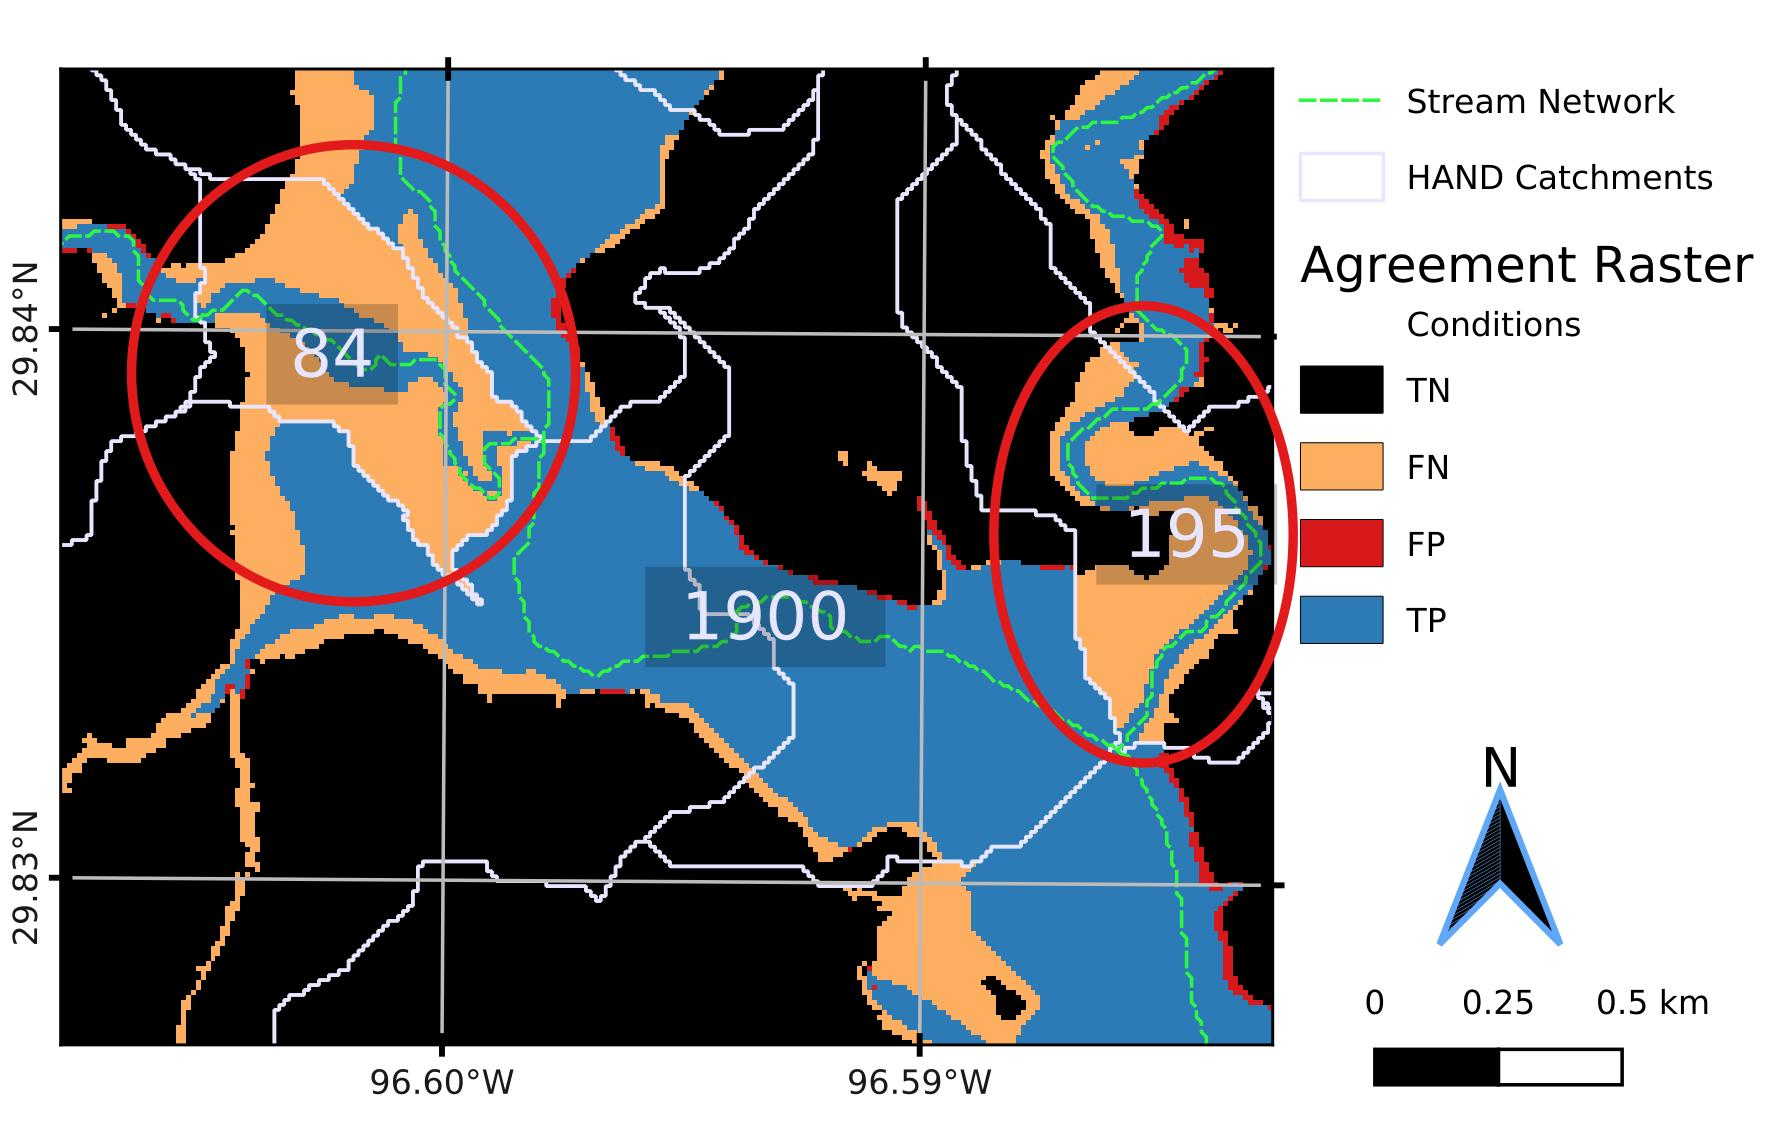
\includegraphics[scale=1.0]{figures/catchment_boundaries_issue.jpg}
\caption{The figure represents an agreement map between a HAND derived FIM and one produced from the Base Level Engineering (BLE) program for a 100yr magnitude event at HUC8 12090301.
Agreement maps are symbolized by false negatives (FN), true negatives (TN), false positives (FP), and true positives (TP) where inundated represents the postive condition (see Section \ref{ssec:evaluation} for more details).
The stream flows associated with each river segment are shown in CMS while the flow directions are symbolized as red arrows.
The presence of FNs at the confluence of tributaries (circled in red) with the main segment is associated with lower flow rates in the tributaries that don't account for backwater effects.
Additionally, the flow of 1900 CMS from the main segment cannot extend to the neighboring catchments belonging to its tributaries shown here.
Water pools up vertically along the catchment boundaries of the higher order segment distorting rating curve behavior (Section \ref{sec:discussion}).
Sourcing fluvial inundation from HAND is limited to only its nearest drainage line which is the main issue this study aims to address.
}
\label{fig:catchment_boundaries_issue}
\end{figure}
%

We seek to resolve this catchment boundary problem or nearest drainage limitation by discretizing the target stream network into stream networks of reduced, unit stream order to avoid the constraining of catchments by those belonging to lower order neighbors.
By discretizing the network into stream networks of unit stream order (later defined as level paths), we remove the influence of neighboring catchments that constrain the inundation extent.
This creates much larger and overlapping catchments that can source fluvial inundation from multiple reaches as required by the given river stage at current flow conditions.
We present two successive methods, National Weather Service MS (Section \ref{sssec:nws_mainstems}) and GMS (Section \ref{sssec:generalized_mainstems}), implemented that reduce drainage densities by reducing Horton-Strahler stream orders of the networks employed and test our presented hypothesis that unary stream order networks enhance FIM performance skill with HAND by expanding the nearest drainage definition to increase potential inundation areas.
%
%%%%%%%%%%%%%%%%%%%%%%%%%%%%%%%%%%%%%%%%%%%%%%%%%%%%%%%%
\subsubsection{NWS Main-stems}
\label{sssec:nws_mainstems}
%
The initial attempt at drainage order reduction to solve the catchment boundary issue was to use a stream network relevant to the NWS forecasting community. 
The Mainstems (MS) network is a subset of the NWM full-resolution (FR) network at and downstream of AHPS forecast points as seen in Figure \ref{fig:forecast_points}.
The MS network comprises about 200 thousand km of stream length which is less than 4\% of the FR total stream length of 5.5 million km.
It also spans 121,724 reaches across 1,608 HUC8s.
In this technique, we derive HAND using the FR stream network as well as the MS network which was originally proposed by \citeA{djokic2019arc}.
Inundation is derived independently from the resulting FR and MS HAND hydrofabric are mosaiced together using the technique proposed in Section \ref{ssec:inundation_mapping} to form the MS FIMs. 
Within each HUC, you'll typically only find a MS stream network of stream order 1 (i.e. headwater) but this can vary if more than one AHPS forecasting point is found within or upstream of the HUC in question.
So while we may refer to the MS network as that of one with unit stream order, we acknowledge there are many cases where additional or converging forecast points create multiple branches within a given processing unit.
%
%%%%%%%%%%%%%%%%%%%%%%%%%%%%%%%%%%%%%%%%%%%%%%%%%%%%%%%%
\subsubsection{Generalized Mainstems}
\label{sssec:generalized_mainstems}
%
Since MS only covers 4\% of the entire FR stream network, we sought to expand drainage order reduction techniques to all reaches within the NWM modeling domain.
In order to do this, we discretized the NWM network into level paths which when considered individually have unit Horton-Strahler stream orders thus significantly reducing drainage density.
Level paths group flowlines by maximizing the length of each flow path and minimizing the number of level path identifiers within a given domain \cite{moore2019user,mckay2012nhdplus}. 
Starting at the outlet, a unique level path is propagated upstream. 
At every confluence, the direction of maximum flow path length is sought to propagate the current level path identifier.
For the remaining parent reaches of the given junction, a new level path identifier is assigned and the process recursively continues with them.

Figure \ref{fig:level_path_methods} illustrate how level paths (symbolized by unique colors) are propagated upstream by the value of arbolate sum.
Each HUC8 is discretized into level paths independently and relevant inputs are assigned to each level path processing unit given a buffer of 7 km.
This buffer was selected to avoid edge contamination \cite{lindsay2013measuring} and to ensure adequate data availability for wide rivers with large catchments in regions with low slope.
Further work could be dedicated to tune this user exposed parameter to better balance its effect on FIM extents and computational expense since larger buffers create additional floating points and calculations to process and store.
At the level path scale, the methods in Sections \ref{ssec:hydro_conditioning} and \ref{ssec:deriving_fim_hydrofabric} are executed leaving out any tributaries of the level path in question at the time.
The only exception to this is the use of the NWM stream network directly for use with hydro-enforcement which was motivated by the difficulty in deriving level paths in the NWM stream network with high agreement with the NHDPlusHR stream lines.
Once the NWM FR stream network is discretized into level paths, we independently compute HAND using each level path as the target stream network to be used.

To illustrate the GMS procedure, we reference Figure \ref{fig:gms_methods} to show how deriving HAND and FIMs from GMS works.
In Figure \ref{fig:gms_methods}a, we uniquely color code the level paths derived for the NWM stream network. 
For each one of these lines, we derive HAND and its associated datasets including catchments, crosswalks, and rating curves.
Each level path is buffered to a polygon with a user-available distance parameter of 7 km and this polygon is used to subset the original DEM for two selected level paths in Figure \ref{fig:gms_methods}b.
We illustrate two HAND grids for two of the level paths in this HUC8 in Figure \ref{fig:gms_methods}c.
Once the FIM hydrofabrics for each level path are generated, we can inundate them individually also shown in Figure \ref{fig:gms_methods}d.
Lastly, these individual FIMs are mosaiced together as explained in Section \ref{ssec:inundation_mapping} and shown in Figure \ref{fig:gms_methods}d.

For a more intimate look at the drainage order reduction procedure and its effects, GMS, we allude to Figure \ref{fig:gms_methods_2} which references the same area (in HUC8 12090301) and set of river junctions as in Figure \ref{fig:catchment_boundaries_issue}.
The catchments and stream lines for HAND computed at the FR scale are illustrated in Figure \ref{fig:gms_methods_2}a where the respective inundation (for 100 yr magnitude) is heavily constrained by the limited catchment extents especially at junctions.
In subsequent sub-figures, we show the same datasets for the HAND computation problem for this region but discretized into independent level paths for the main level path (b), the eastern tributary (c), and the western tributary (d).
Notably, inspecting (b) one sees how removing the tributaries creates much larger catchments for the main level path. 
These catchments include drainage areas that would traditionally be considered nearest to the tributaries thus ineligible to receive inundation sourced from the main level path.
The inundation extents in (b) overlap those of (c) and (d) and are mosaiced together by methods explained in Section \ref{ssec:inundation_mapping}.
%
\begin{figure}[h!]
\centering
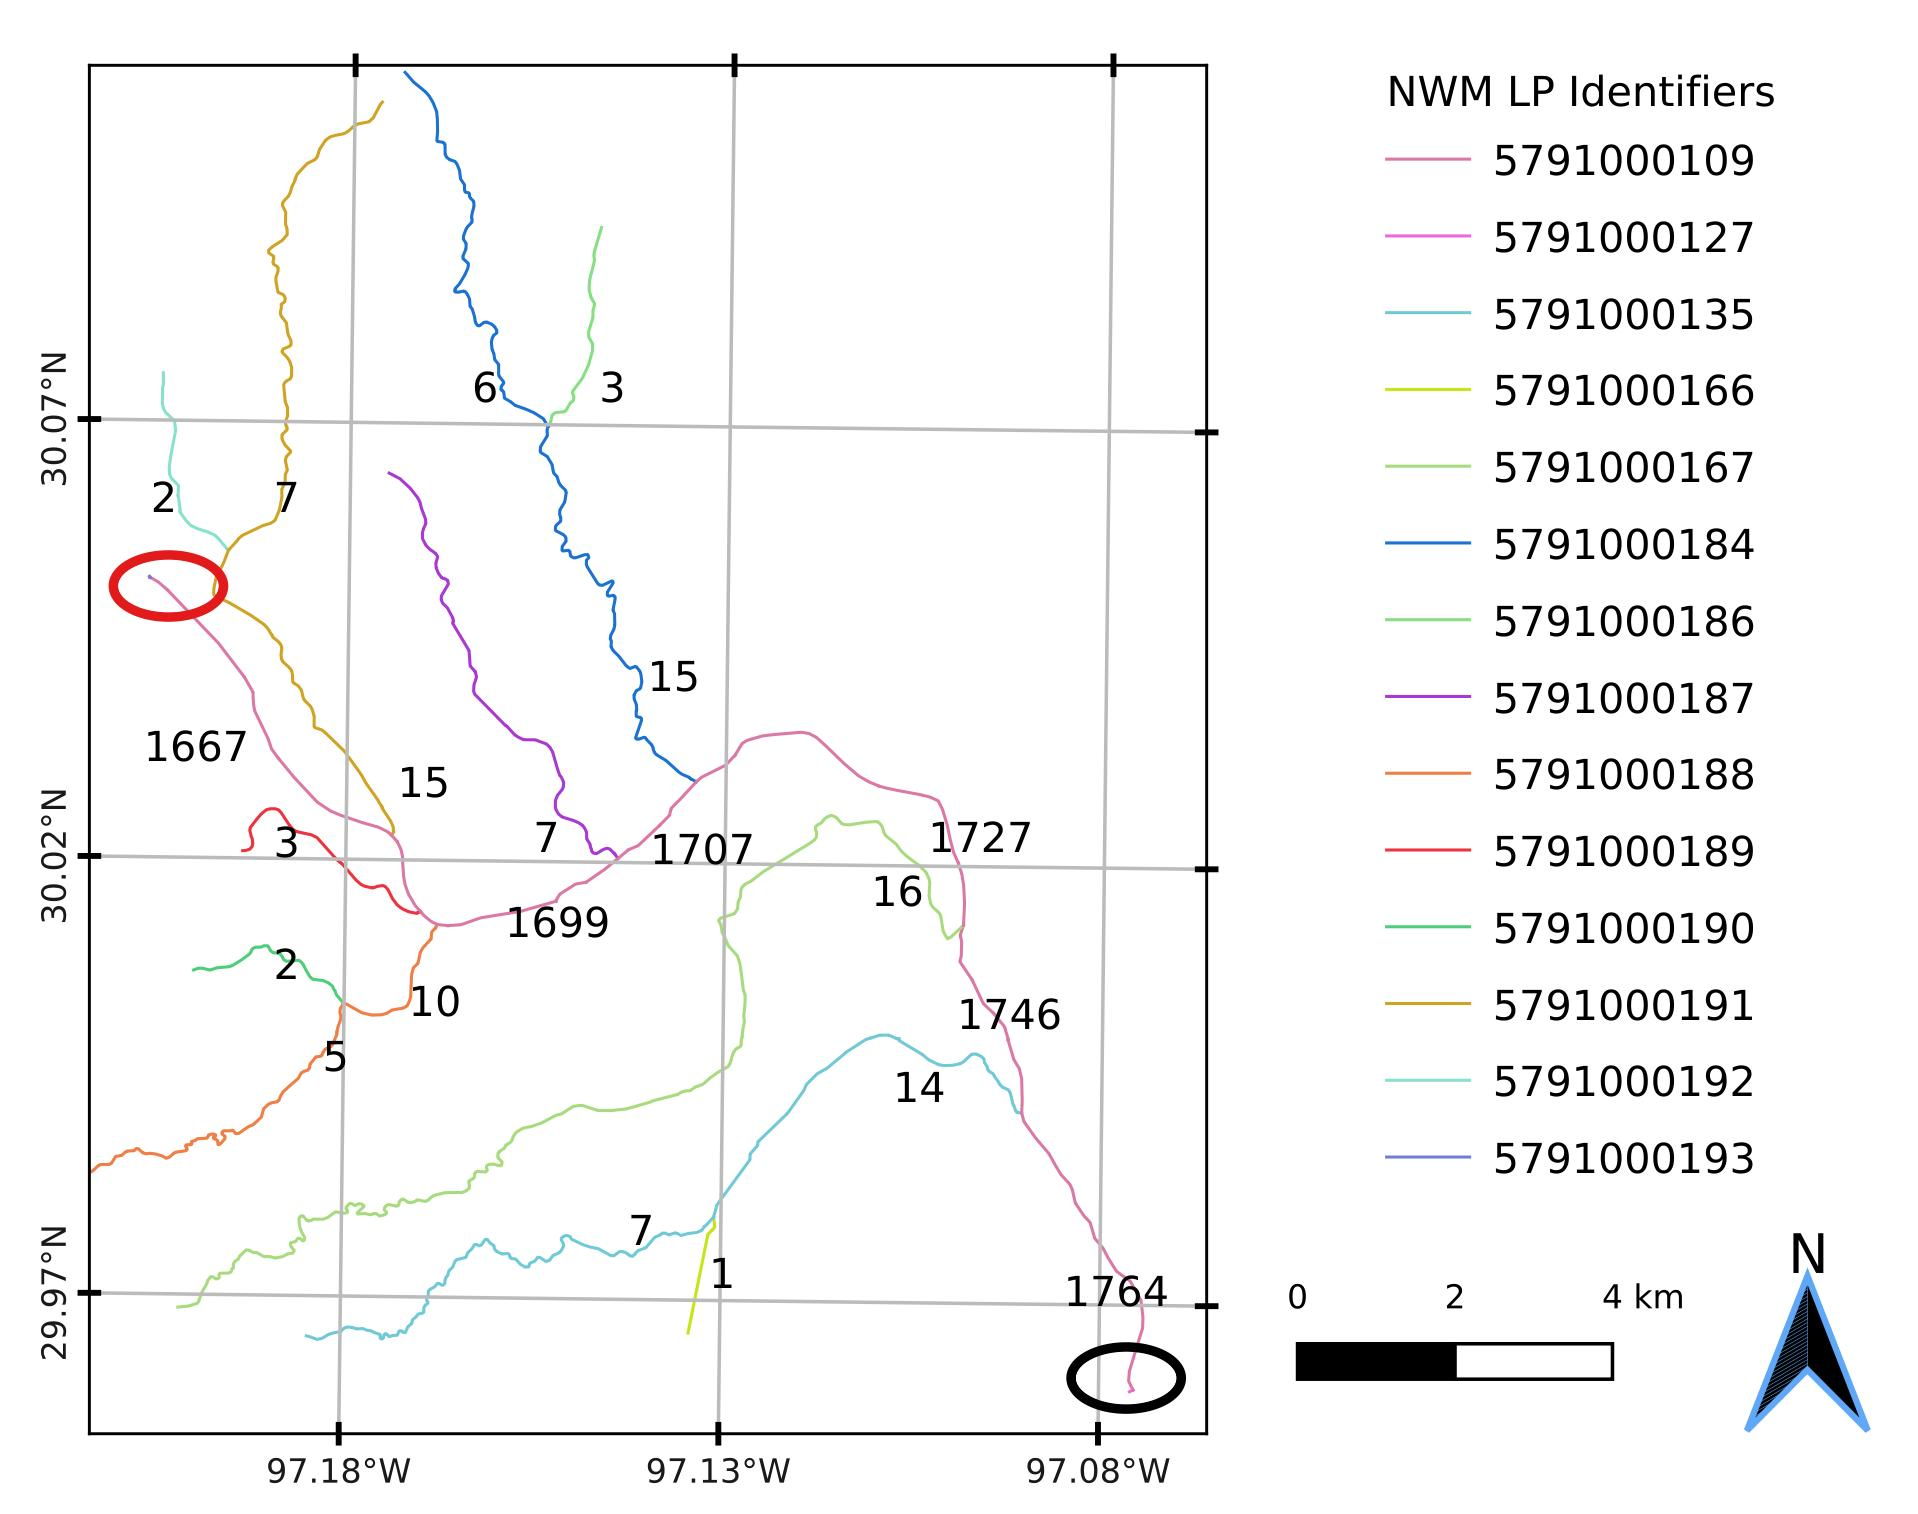
\includegraphics[scale=1.0]{figures/level_path_methods.jpg}
\caption{Illustrates how level paths (LP) for the NWM stream network are derived.
They are derived by starting at an outlet point with a unique ID which are symbolized by unique colors.
Once a junction is reached, the current level path identifier is propagated in the direction of highest arbolate sum.
The remaining converging members at the given junction are each assigned a new unique LP identifier and the process is repeated recursively until all reaches have been assigned a level path.
The values shown labeling the reaches above are arbolate sums which is defined as the cumulative distance of all upstream reaches.
Thus, level paths serve as a proxy means of assigning membership to a given river when presented with a confluence.
Each individual level path has a unit Horton-Strahler stream order thus serves as a great method for our proposed technique.
}
\label{fig:level_path_methods}
\end{figure}
%
%
\begin{figure}[h!]
\centering
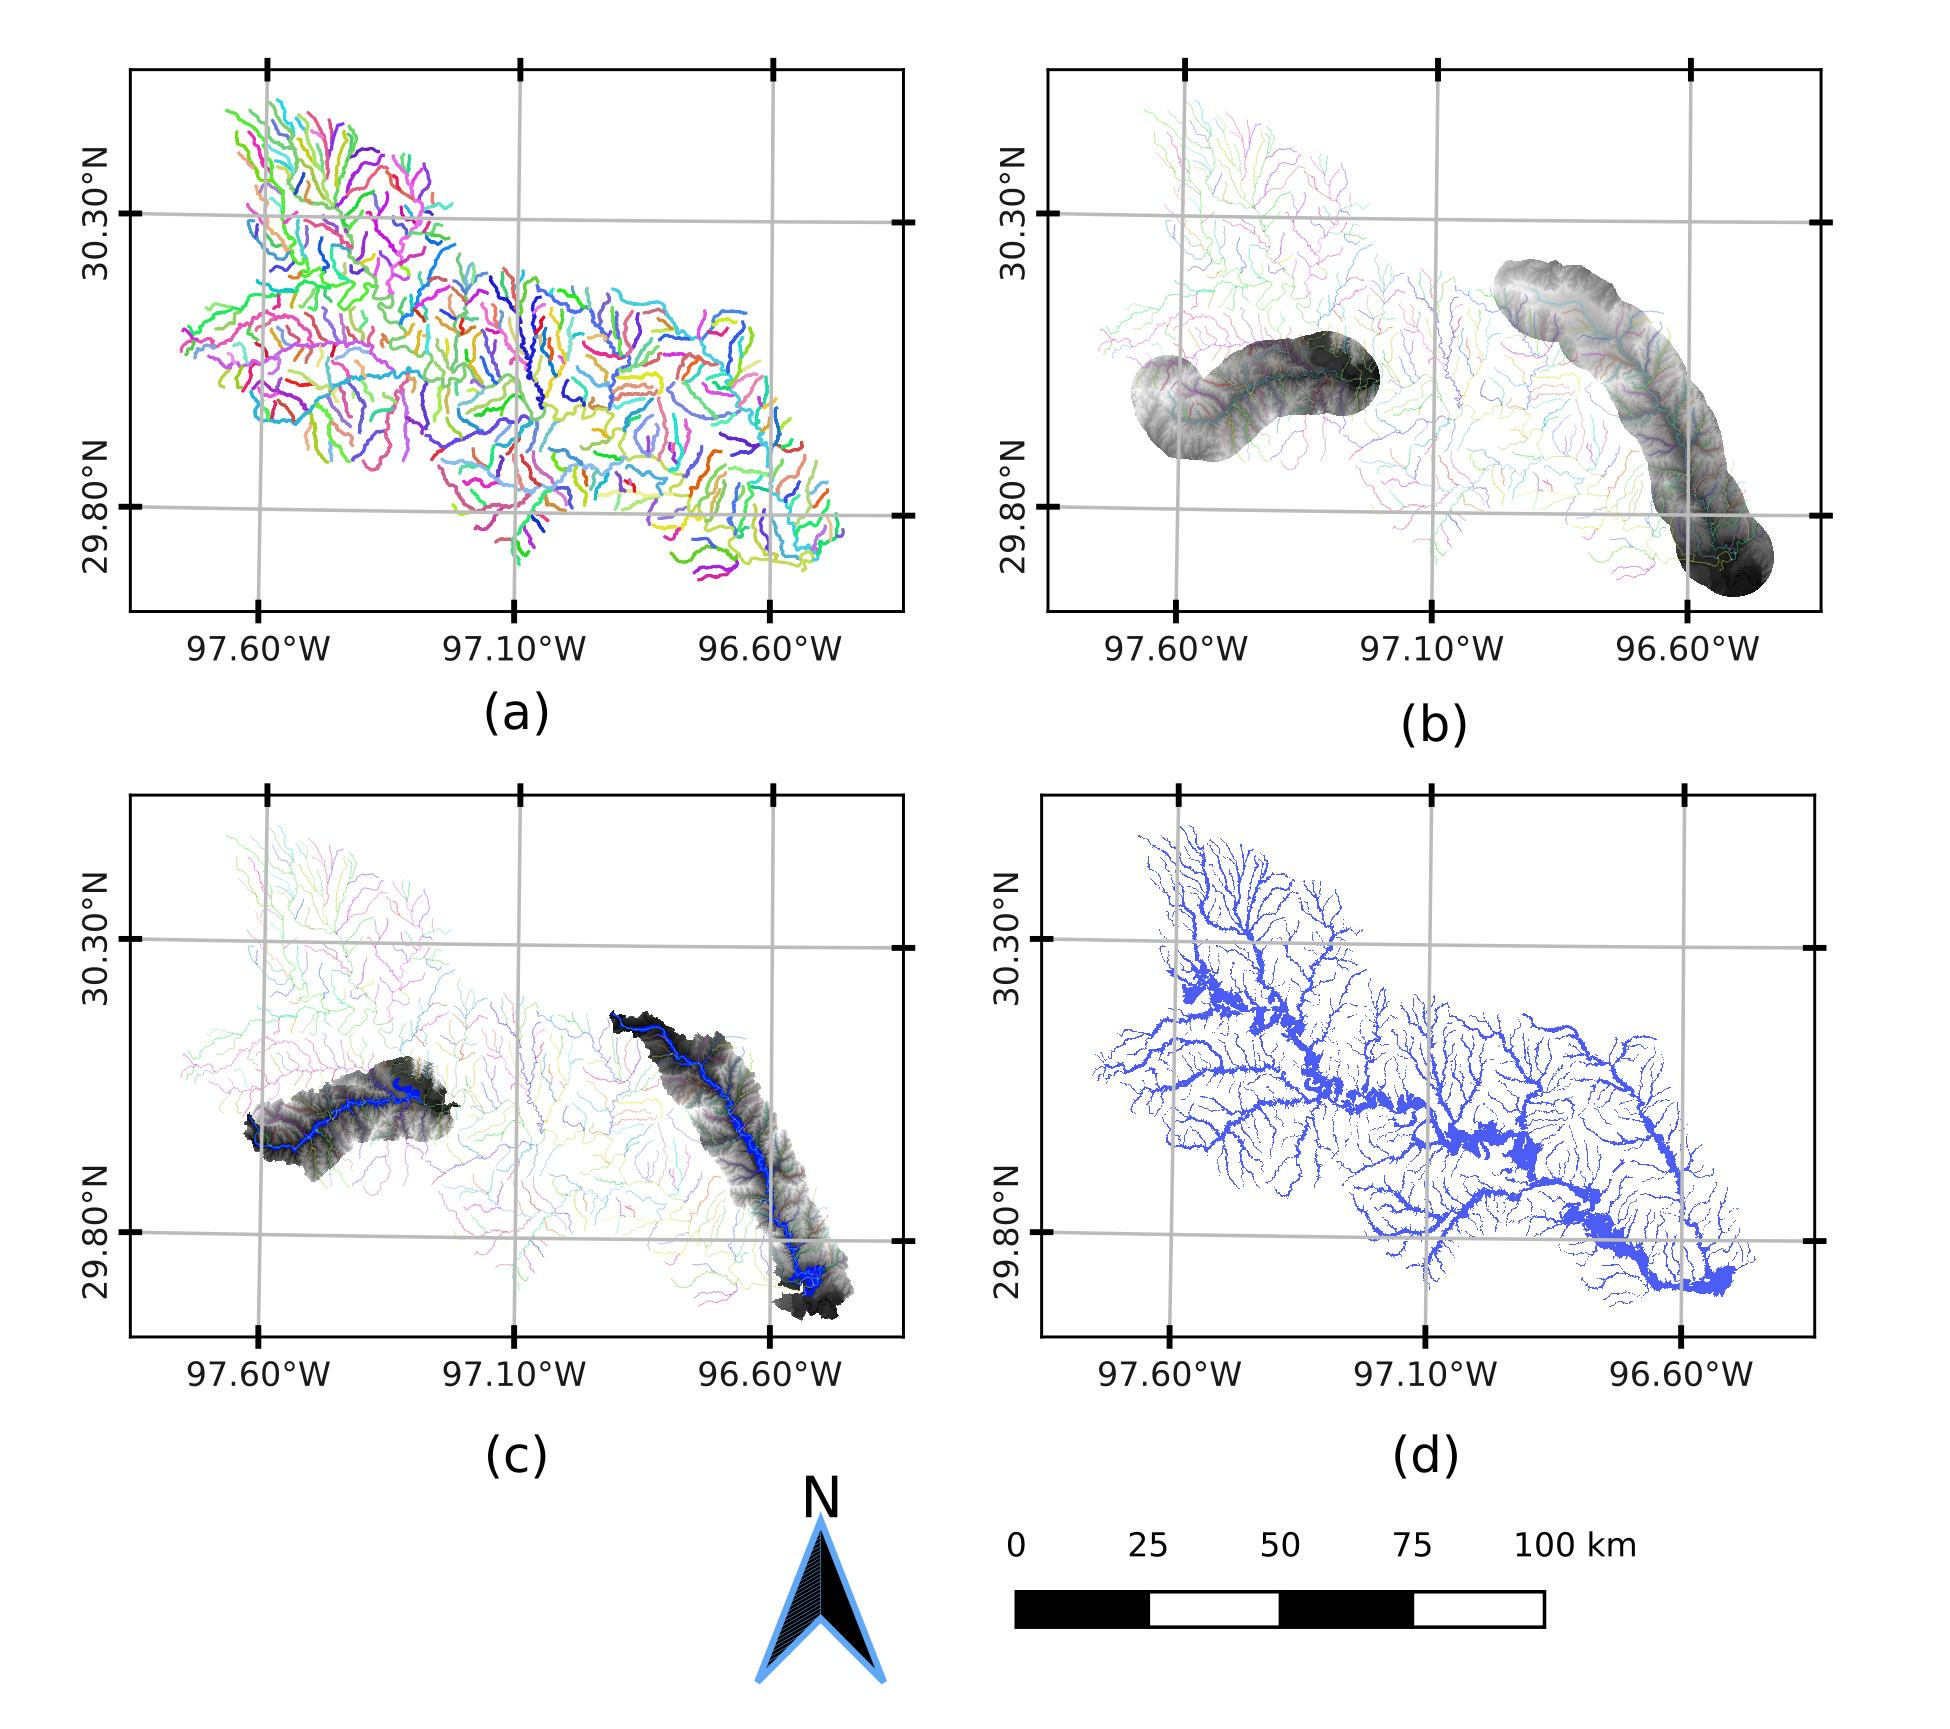
\includegraphics[scale=1.0]{figures/gms_methods.jpg}
\caption{Overall procedure for GMS HAND at HUC8 12090301.
In (a), we illustrate all NWM stream lines symbolized by their level path with 372 unique level path IDs in this HUC.
Meanwhile (b), demonstrates the DEM clipped to a 7 km buffer around two selected level paths.
In (c), we show how HAND can be computed just for each one of these two level paths independently. 
We also show inundation maps created for these two level paths in (c). 
In (d), we show all the inundation maps for all the level paths mosaiced together. }
\label{fig:gms_methods}
\end{figure}
%
%
\begin{figure}[h!]
\centering
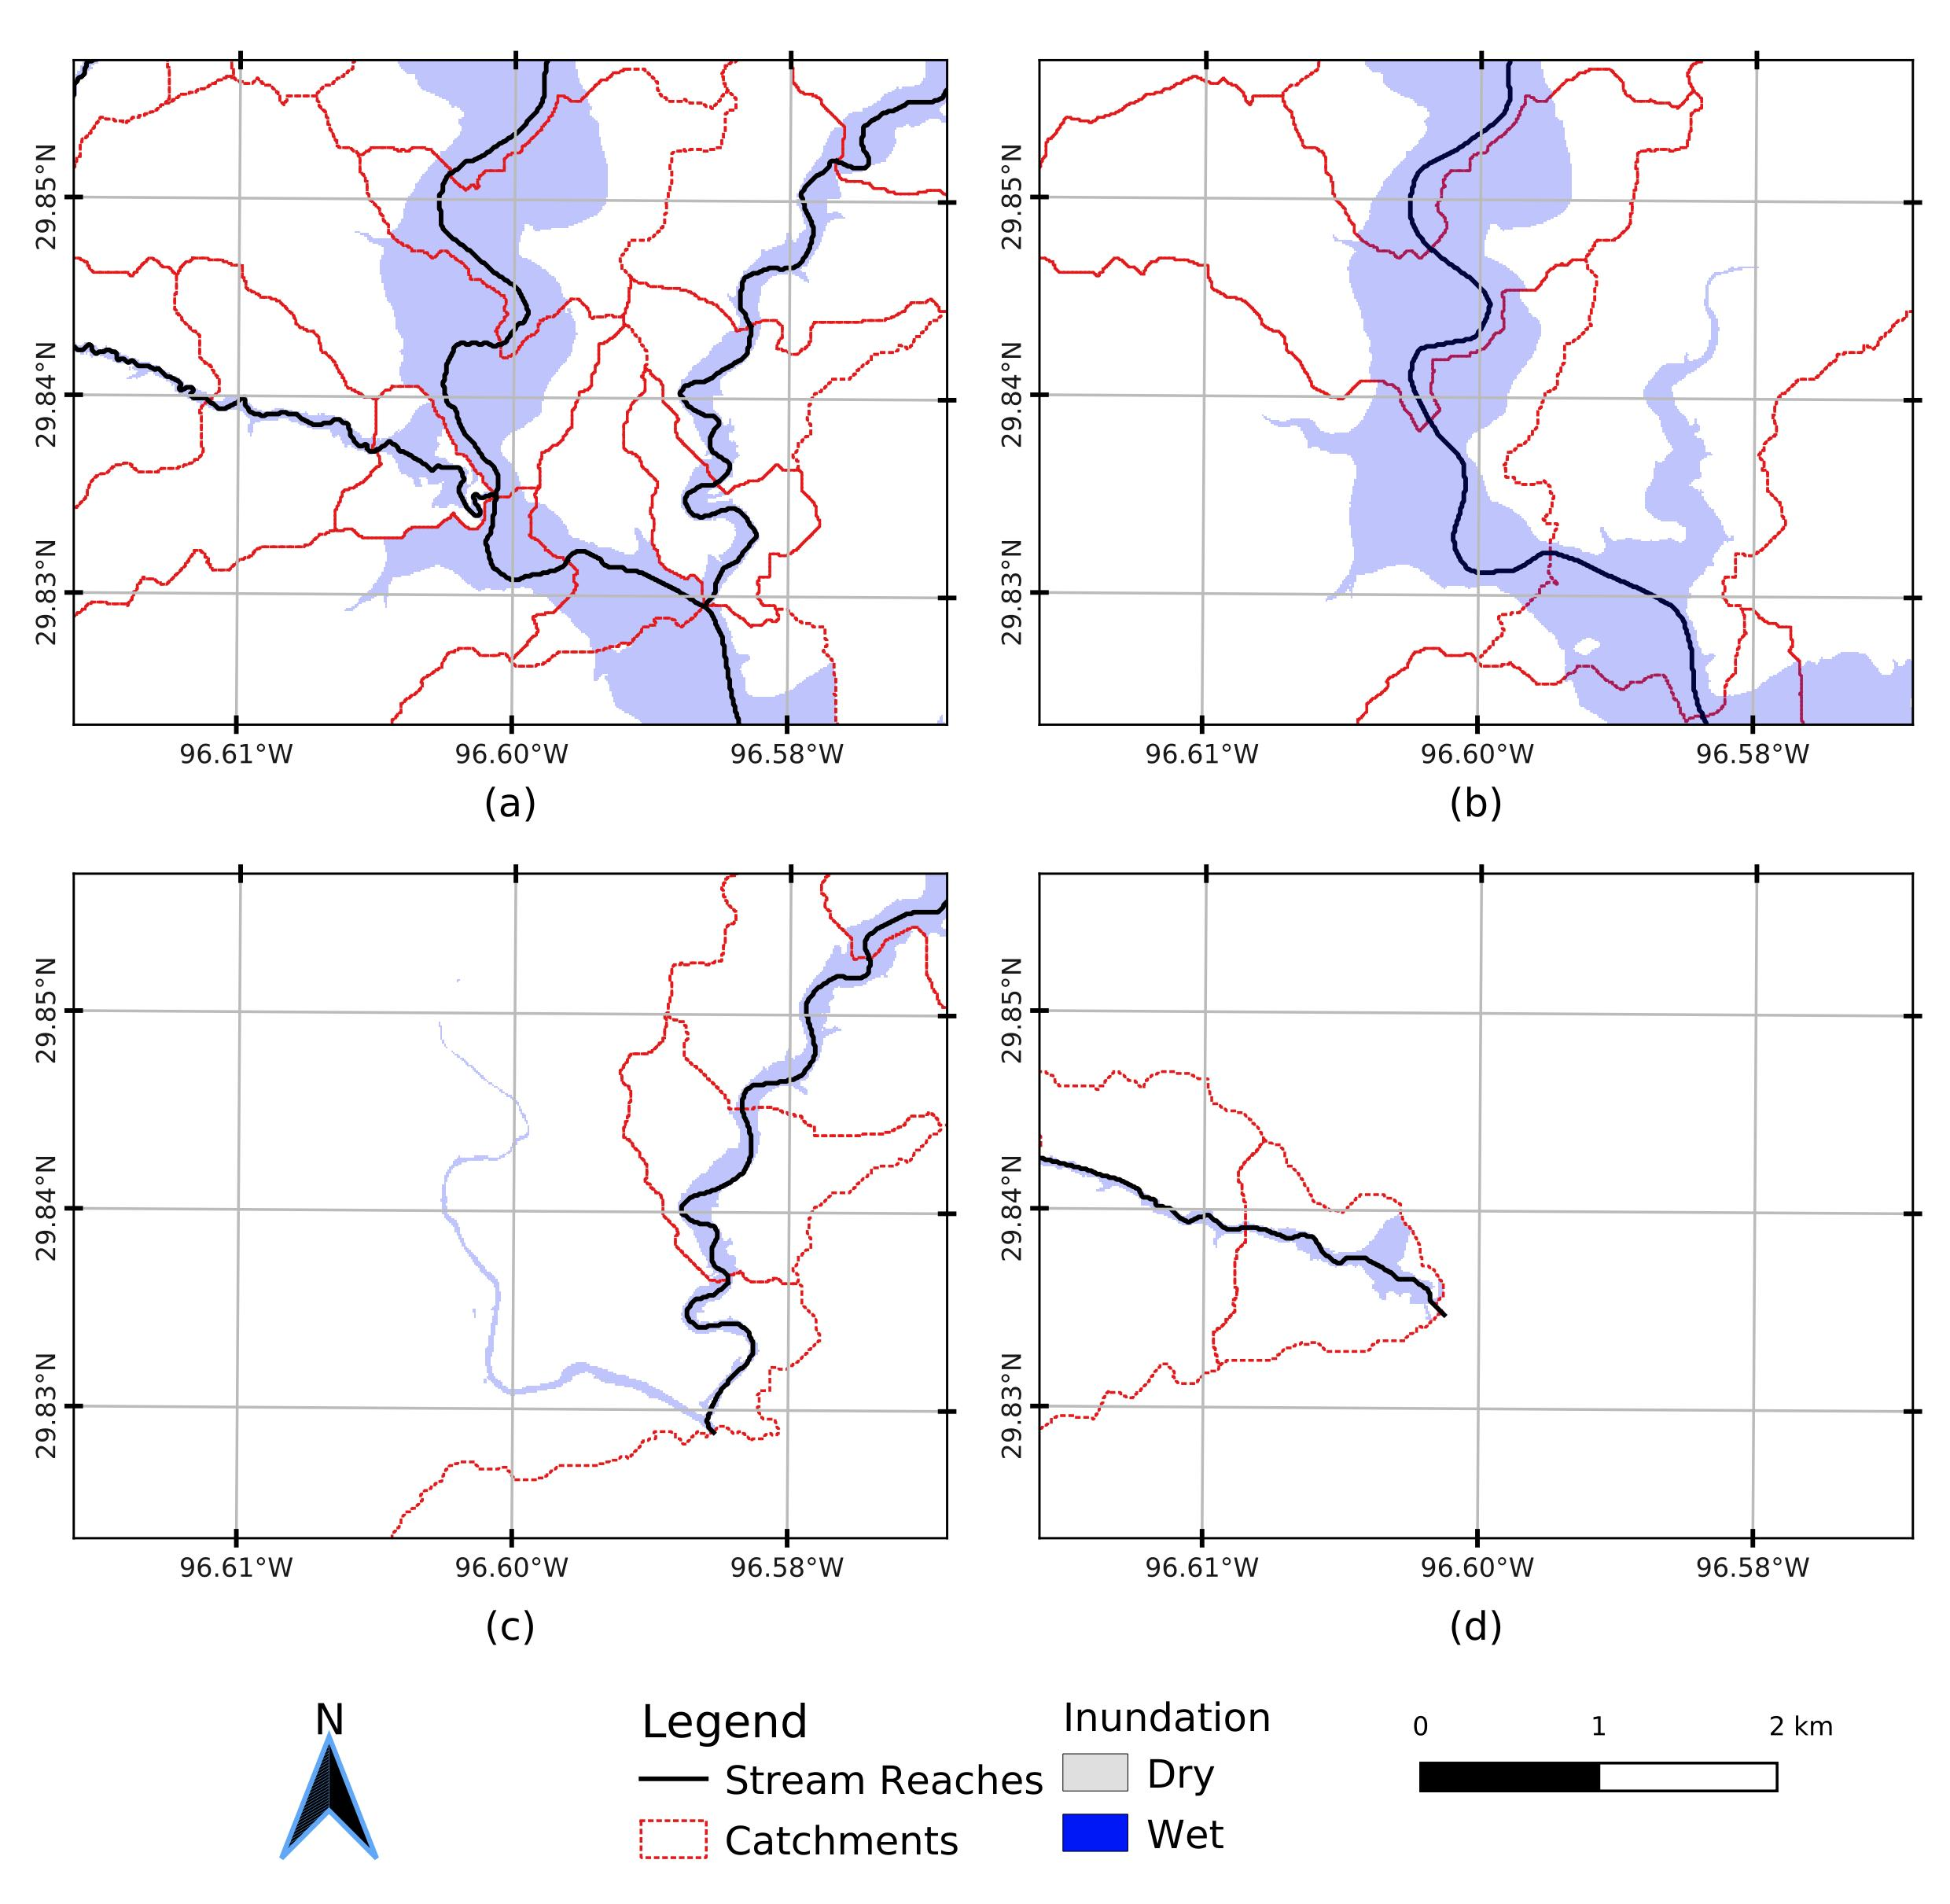
\includegraphics[scale=0.70]{figures/gms_methods_2.jpg}
\caption{This image, with the same spatial domain as Figure \ref{fig:catchment_boundaries_issue} (HUC 12090301), demonstrates how computing HAND on level path bases leads to larger, independent catchments and more expansive inundation extents (100 yr flows).
In (a), the catchments and stream network are shown for HAND computed in Full-Resolution (FR) method which shows constrained inundation extents around the two junctions.
(b) demonstrates the level path associated with this region's highest order river.
By delineating catchments at this scale indepedent of the neighboring tributaries, the drainage areas are allowed to expand thus allowing inundation extents to cover previously restricted areas.
In (c) and (d), we show the stream lines, catchments, and inundation extents of the two tributaries.
Later in Section \ref{ssec:inundation_mapping}, we describe how the inundation in (b), (c), and (d) are mosaiced together to form one seamless inundation map.
This process allows for multiple, possible contributing sources of fluvial inundation to be considered thus enhancing FIM skill.
}
\label{fig:gms_methods_2}
\end{figure}
%
%%%%%%%%%%%%%%%%%%%%%%%%%%%%%%%%%%%%%%%%%%%%%%%%%%%%%%%%
\subsection{Inundation Mapping}
\label{ssec:inundation_mapping}
%
The FIM hydrofabric consisting of the relative elevations grid, catchments grid, catchment polygons, rating curve, and cross-walking data are all used to convert forecasts from the NWM into forecasts extents.
For operational situations, one would cache the FIM hydrofabric then either produce libraries of FIM for a sample of discharges or stages or also produce the FIM in near real-time (NRT).
From the cached FIM hydrofabric and design or forecast discharges including those extracted from the NWM, inundation maps can be generated at HUC 8 spatial processing units in a rapid, parallel operation. 
The discharges are associated with NWM reach identifiers and cross-walked over to reach identifiers in the FIM hydrofabric.


Utilizing the stage-discharge relationships in the synthetic rating curves, each forecast for each catchment identifier is assigned a stage value. 
The catchments grid encoded with the reach identifiers are used to map the stages by thresholding to the forecast stage.
We use the basic logic already established in previous works to conduct this \cite{nobre2016hand,liu2016cybergis,maidment2017conceptual}.
Mathematically, the HAND values, $H_{ij}$, can be indexed by the reach identifiers, i, and pixel indices, j.
For each forecast stage, $S_i$, one can express the formula for $D_{ij}$, a continuous variable denoting water depth at a given pixel with reach and pixel identifiers i and j respectively in Equation \ref{eq:hand_fim_depth}.
For each forecast stage, $S_i$, one can express the formula for $F_{ij}$, a binary variable denoting inundation condition in Equation \ref{eq:hand_fim} in terms of $D_{ij}$ by simply thresholding at zero depths.
%
\begin{linenomath*}
\begin{equation}
\label{eq:hand_fim_depth}
    D_{ij} = S_i - H_{ij}
\end{equation}
\end{linenomath*}
%
\begin{linenomath*}
\begin{equation}
\label{eq:hand_fim}
    F_{ij} = D_{ij} > 0
\end{equation}
\end{linenomath*}
%
For the cases of MS and GMS, the inundation maps produced for the respective processing units at lower maximum stream orders must be mosaiced together to form a seamless forecast in the form of a single raster file.
For mosaicing the depths, we select the maximum inundation depth from the all the contributing areas K index by its lower case character, k.
Consolidating the depths using a maximum function was decided upon based on intuition which we believe to best represent the depth of water in an area with multiple contributing fluvial inundation sources.
Other aggregation methods could lead to different results but were not investigated here.
Equation \ref{eq:comp_fim_depths} illustrates how the maximum depth from all the contributing areas, k, to each pixel j in catchment i.
Equation \ref{eq:comp_fim} illustrates the same process but for mosaicing the binary inundation maps.
%
\begin{linenomath*}
\begin{equation}
\label{eq:comp_fim_depths}
    D_{ij} = \max_{k=[1,...,K]} D_{ijk}
\end{equation}
\end{linenomath*}
%
For the MS and GMS methods, the contributing areas are defined differently.
For MS, the FIM from MS HAND and FR HAND are mosaiced together to form a singular inundation map thus K is set to 2 for that case.
For GMS, all FIMs from all the level paths in a given area are mosaiced together then K is set to this number of level paths.
Figures \ref{fig:gms_methods}a and \ref{fig:gms_methods}b, illustrate how inundation maps are created for lower stream order processing units then mosaiced together.
%
\begin{linenomath*}
\begin{equation}
\label{eq:comp_fim}
    F_{ij} = \max_{k=[1,...,K]} F_{ijk}
\end{equation}
\end{linenomath*}
%
%%%%%%%%%%%%%%%%%%%%%%%%%%%%%%%%%%%%%%%%%%%%%%%%%%%%%%%%
\subsection{Evaluation}
\label{ssec:evaluation}
%%%%%%%%%%%%%%%%%%%%%%%%%%%%%%%%%%%%%%%%%%%%%%%%%%%%%%%%
%
Possible benchmark FIM candidates for evaluation purposes include high-water marks, remote sensing observation, crowd-sourced information, and modeled extents.
Unfortunately, all of these sources or using a combination of them are subject to limitations for evaluating a continental scale model like OWP FIM such as but not limited to lack of spatial coverage, signal interference, lack of stream flow data, inaccurate stream flow data, physics-based assumptions, and errors in input data.
While in-situ observations such as high water marks offer the highest accuracy, they are often limited in spatial extent and can lack the associated stream flow data necessary to make FIMs to compare to.
A suitable dataset needed to be selected to best balance advantages and limitations with future studies interested in expanding to additional datasets as able to.

Evaluation of our relative elevation CFIM method is conducted by comparison to the HEC-RAS 1D derived models produced within FEMA region 6 \cite{fema2021base,fema2021estimated}.
This dataset was selected due to its large spatial coverage, availability of cross-sections with stream flow information, more sophistication when compared to HAND based FIMs, engineering scale detail, and a storied use in the literature as an evaluation dataset \cite{cook2009effect,rajib2016large,zheng2018geoflood,afshari2018comparison,wing2017validation,criss2022stage,follum2017autorapid}.
49 HUC 8's spanning about 185 thousand square km were available at the time (now more) across nine states and shown in Figure \ref{fig:all_ble_maps}.
The maps to the 1\% recurrence flow (1 in 100 year) and the 0.2\% recurrence flow (1 in 500 year) are furnished by InFRM so we used those corresponding discharges and mapping extents for evaluation.
We did exclude NWM V2.1 Reservoirs from evaluation because these are not properly accounted for in the inundation.

By using the same HEC-RAS derived discharges and FIM extents, we are able to separate out errors introduced by hydrology, atmospheric forcings, hydraulic routing, etc that we would have potentially seen if we used NWM forecasted discharges.
Figure \ref{fig:ble_evaluation_method} illustrates both NWM V2.1 and BLE stream lines as well as the BLE cross-sections that have recurrence discharges associated with them.
We elected to spatially intersect the HEC-RAS cross sections with the NWM stream network assigning the 1\% and 0.2\% flow rates to each NWM reach. 
To handle multiple intersections, we opted to use a filter to select the median discharge value attributed to each NWM reach.
This partially handles the influence of neighboring cross sections that could cause flow discontinuities and mass conservation issues.
Additionally, the stream network of the InFRM furnished models are of higher stream densities and bifurcation ratios, as evident in Figure \ref{fig:ble_evaluation_method}, leading to a significant amount of false negatives (FN) (under-prediction) along headwater streams with Horton-Strahler orders of one due to the lack of representation of these additional headwater streams in the NWM network.
While the limitations are noted, this method does best to detangle the influence of exogenous variables that we do not wish to study in this comparison.
%
\begin{figure}[h!]
\centering
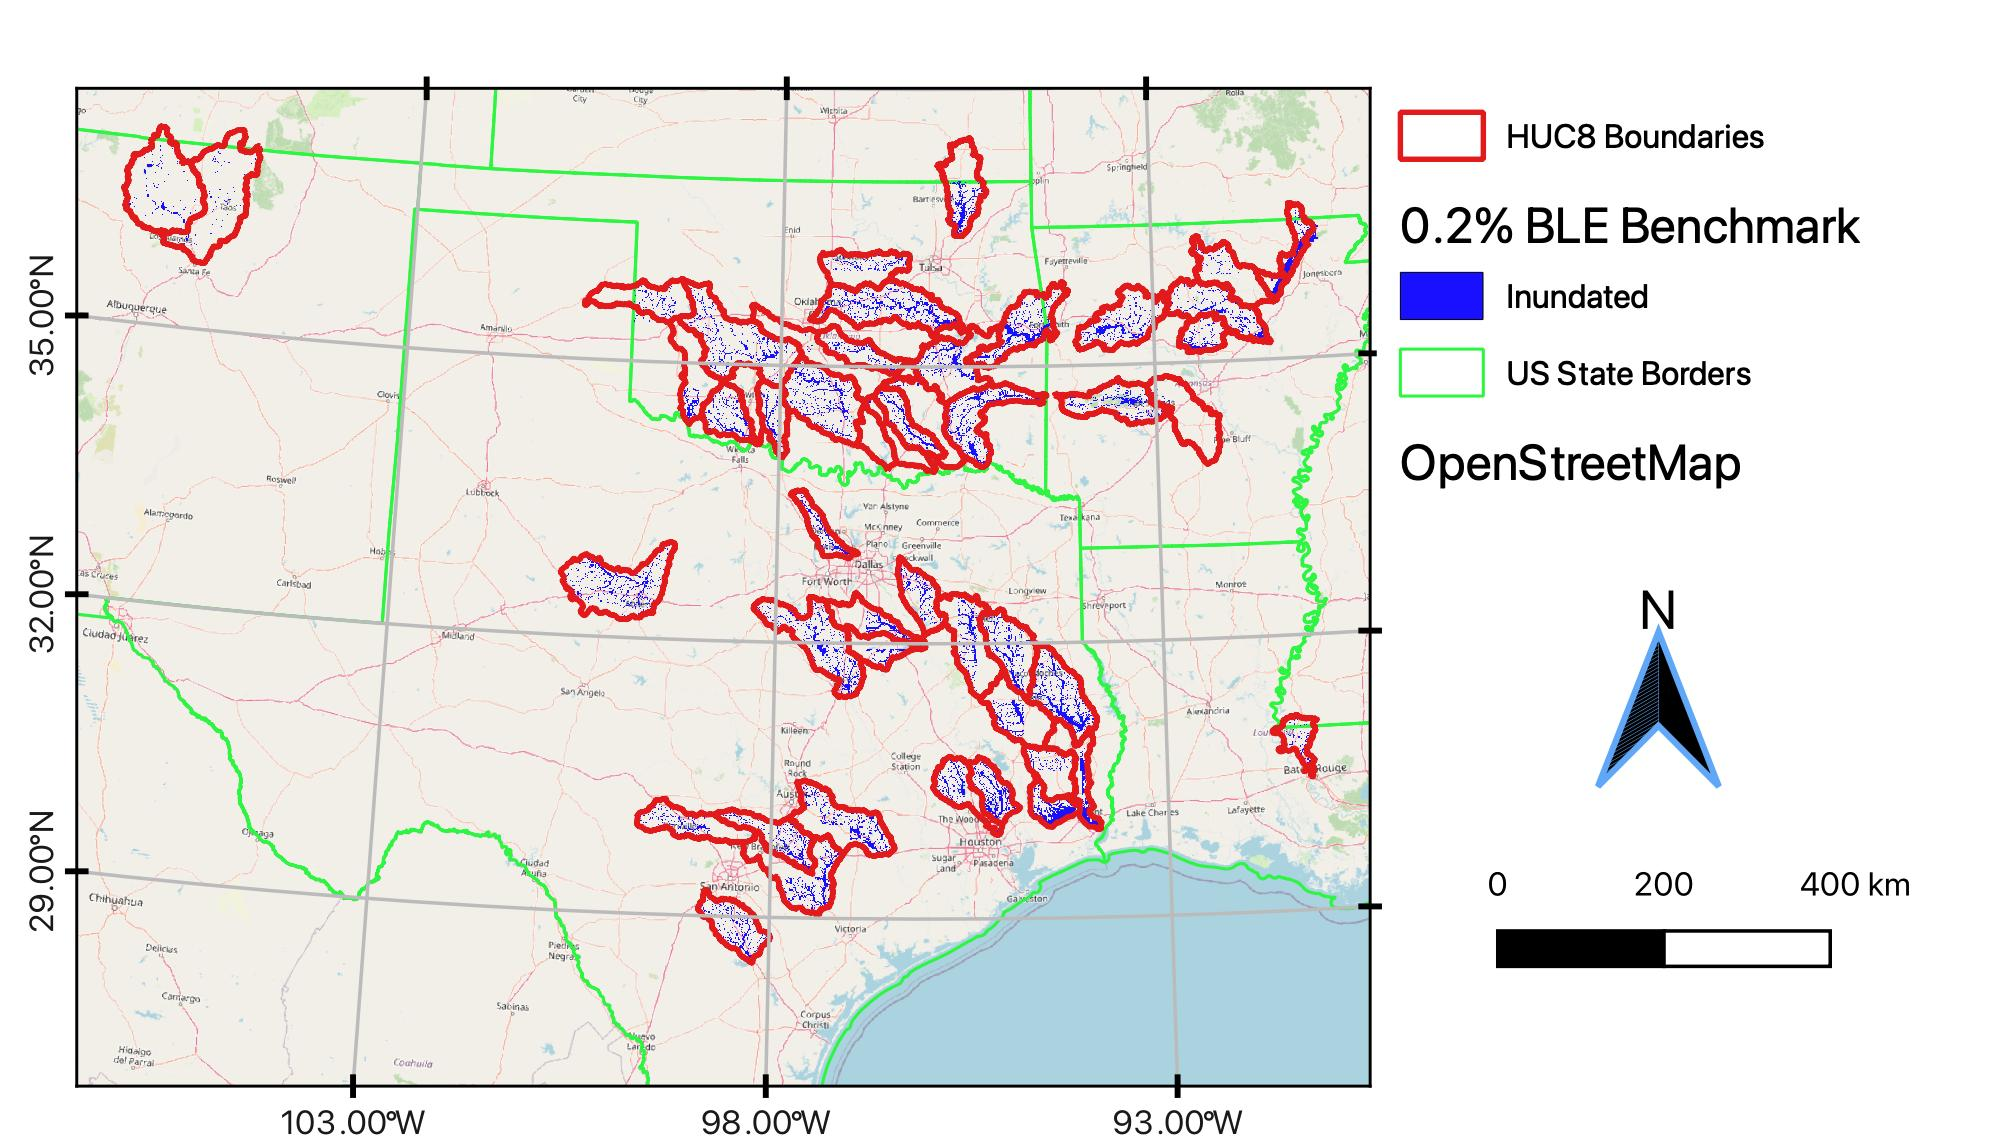
\includegraphics[scale=1.0]{figures/all_ble_maps.jpg}
\caption{Shows 185 thousand square km of modeled areas for BLE domain of 49 HUC8s across 9 states at 0.2\% recurrence magnitude for flow rates.}
\label{fig:all_ble_maps}
\end{figure}
%
\begin{figure}[h!]
\centering
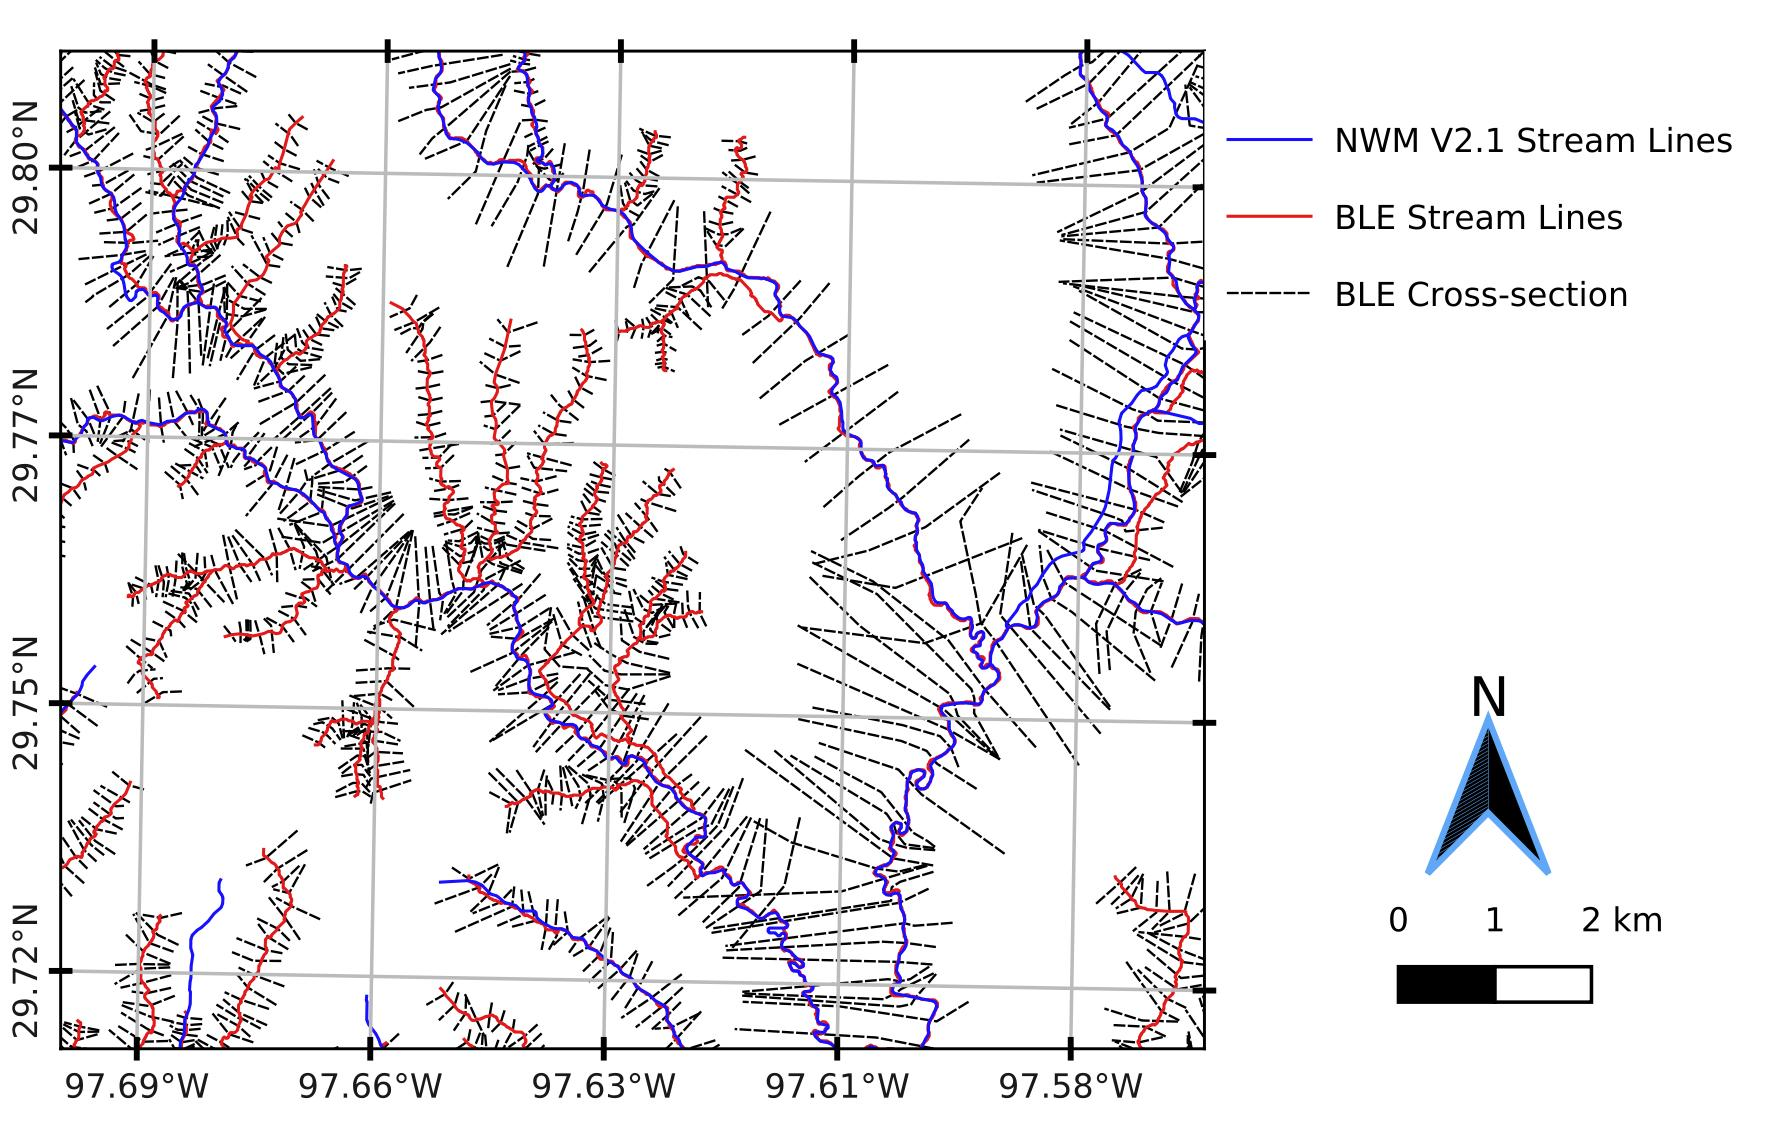
\includegraphics[scale=1.0]{figures/ble_evaluation_method.jpg}
\caption{
Illustrates Base Level Engineering (BLE) cross sections and stream lines at the HUC8 12100203 near the confluences of West Fork Plum Creek and Clear Fork Plum Creek with Plum Creek.
BLE cross sections are intersected with NWM reaches and the median recurrence discharge for 1\% and 0.2\% levels are selected per NWM V2.1 Full Resolution (FR) stream lines.
Additionally, we illustrate the NWM V2.1 catchments to provide a sense of how many cross-sections may intersect a given NWM flow line.
The BLE stream network is also shown which is denser than the NWM V2.1 stream lines meaning there are several lower order streams represented in the BLE stream network that are not in the NWM V2.1 stream lines.
This creates additional inundation areas in the validation data that are not modeled with our HAND based FIMs.
}
\label{fig:ble_evaluation_method}
\end{figure}
%

The metrics employed in this study to evaluate inundation extents include Critical Success Index (CSI), Probability of Detection (POD), and False Alarm Ratio (FAR) and presented in Equations \ref{eq:csi}, \ref{eq:pod}, \ref{eq:far}, respectively.
To calculate these secondary metrics, one must define three primary metrics including true positives (TP) which is predicted wet and wet in benchmark dataset.
The two types of errors consist of false positives (FP), or type I errors, which is dry in benchmark but predicted wet and false negatives (FN), or type II errors, which is wet in benchmark by predicted dry. 
Lastly, the reader may come across true negatives (TN) which is defined as dry in both the benchmark and predicted datasets.
Some work by \citeA{gerapetritis2004behavior} while at the NWM denotes CSI a good proxy for measuring a forecasting system's utility in protecting life and property and has been shown to be optimized mathematically when $POD = 1 - FAR$.
Maximizing POD indicates a model's ability to detect the given threat of interest, inundation, while minimizing FAR is sought to indicate a models ability in reducing FN errors.
In other words, POD is an indicator of model skill in inundated regions while FAR is an indicated of model skill in non-inundated regions.
We use all three secondary metrics here to add value to the discussion while avoiding aggregating away the meaning of all four primary metrics.

While these metrics are commonly employed in the evaluation of FIM and binary weather prediction communities in general, they do come with some notable limitations including frequency dependence in the case of CSI and FAR \cite{gerapetritis2004behavior,stephens2014problems,schaefer1990critical,jolliffe2012forecast}.
Thus, frequency dependent statistics should be used with caution when comparing across sites with varying frequencies. 
Lastly, approximately 6 HUC8s do not have NWM MS reaches thus we imputed the metrics for FR for these sites as the best available forecasting capability.
%
\begin{linenomath*}
\begin{equation}
\label{eq:csi}
CSI = \frac{TP}{TP + FN + FP}
\end{equation}
\end{linenomath*}
%
\begin{linenomath*}
\begin{equation}
\label{eq:pod}
POD = \frac{TP}{TP + FN}
\end{equation}
\end{linenomath*}
%
\begin{linenomath*}
\begin{equation}
\label{eq:far}
FAR = \frac{FP}{TP + FP}
\end{equation}
\end{linenomath*}
%
